\documentclass[11pt,a4paper]{report}

% Page Layout & Geometry
\usepackage[a4paper,top=2.5cm,bottom=2.5cm,left=2.5cm,right=2.5cm,headheight=14pt]{geometry}

% Color Definitions (Clean Academic / Restrained Agricultural Green)
\usepackage[table,xcdraw]{xcolor}
\definecolor{primarygreen}{RGB}{34, 107, 60}     % Forest/Sage accent
\definecolor{darkcharcoal}{RGB}{33, 37, 41}      % Charcoal body text
\definecolor{lightgraybg}{RGB}{248, 249, 250}    % Soft table/box background
\definecolor{bordergray}{RGB}{222, 226, 230}     % Border gray
\definecolor{alertred}{RGB}{185, 28, 28}         % Critical alert red

% Typography & Math Packages
\usepackage{amsmath,amssymb,amsfonts}
\usepackage{bm}
\usepackage{fancyhdr}
\usepackage{booktabs}
\usepackage{longtable}
\usepackage{tabularx}
\usepackage{array}
\usepackage{graphicx}
\usepackage{tikz}
\usetikzlibrary{shapes.geometric,arrows.meta,positioning,calc}
\usepackage{listings}
\usepackage{microtype}
\usepackage[numbers,sort&compress]{natbib}
\usepackage[nottoc]{tocbibind}

% Hyperref Setup
\usepackage[hidelinks,colorlinks=true,linkcolor=primarygreen,citecolor=primarygreen,urlcolor=primarygreen]{hyperref}

% Header and Footer Styling
\pagestyle{fancy}
\fancyhf{}
\fancyhead[L]{\textcolor{gray}{\small\leftmark}}
\fancyhead[R]{\textcolor{gray}{\small FarmShift Nepal — Technical Report}}
\fancyfoot[C]{\thepage}
\renewcommand{\headrulewidth}{0.4pt}
\renewcommand{\footrulewidth}{0pt}

% Code Listings Configuration
\lstset{
  basicstyle=\ttfamily\footnotesize,
  backgroundcolor=\color{lightgraybg},
  frame=single,
  rulecolor=\color{bordergray},
  keywordstyle=\color{primarygreen}\bfseries,
  commentstyle=\color{gray}\itshape,
  stringstyle=\color{darkcharcoal},
  breaklines=true,
  breakatwhitespace=true,
  showstringspaces=false,
  numbers=none,
  tabsize=2
}

\begin{document}

% =========================================================================
% TITLE PAGE
% =========================================================================
\begin{titlepage}
\begin{center}
\vspace*{1.0cm}

{\Huge \bfseries \textcolor{primarygreen}{FarmShift Nepal}}\\[0.5cm]
{\Large \bfseries \textcolor{darkcharcoal}{Technical Architecture, Data Engineering, Agricultural Decision Support, and AI Methodology}}\\[1.2cm]


\begin{tikzpicture}
  \draw[color=primarygreen, fill=primarygreen!8, line width=1.5pt, rounded corners=6pt] (0,0) rectangle (14, 2.5);
  \node at (7, 1.7) {\bfseries \large NASA Space Apps Challenge 2026};
  \node at (7, 1.1) {\textit{Challenge Track: ``Field Shift: Adapting Farms with NASA Data''}};
  \node at (7, 0.5) {\small Domain: Agroclimatology $\cdot$ Earth Observation $\cdot$ Decision Support};
\end{tikzpicture}

\vspace{1.8cm}

\begin{tabular}{rl}
\textbf{Developer / Maintainer:} & Pratik Pokhrel \\
\textbf{Live Application Platform:} & \url{https://farmshift.pokhrelpratik.com.np/} \\
\textbf{Open-Source Repository:} & \url{https://github.com/Spongly/FarmShift} \\
\textbf{Report Version:} & 1.0 (Production Verified) \\
\textbf{Date of Publication:} & October 2026 \\
\textbf{Classification:} & Open-Source Engineering \& Agronomic Specification \\
\end{tabular}

\vfill


\begin{tikzpicture}
  % Subtle decorative satellite / field icon
  \draw[primarygreen, line width=1pt] (0,0) -- (12,0);
\end{tikzpicture}

\vspace{0.4cm}
{\footnotesize \textcolor{gray}{This technical report documents the verified source code, API integrations, and mathematical heuristics of FarmShift Nepal. It is an independent open-source contribution and does not claim official endorsement by NASA or the Government of Nepal.}}

\end{center}
\end{titlepage}

% =========================================================================
% PRELIMINARY PAGES
% =========================================================================
\pagenumbering{roman}

\chapter*{Abstract}
Smallholder farming systems across Nepal's diverse physiographic zones (Terai plains, Mid-Hills, and High Mountains) are increasingly threatened by shifting monsoon onsets, prolonged intra-seasonal dry spells, and chemical nutrient imbalances. \textbf{FarmShift Nepal} is an open-source, client-side agricultural decision-support platform engineered to translate Earth Observation (EO) satellite streams into location-specific, actionable intelligence. Operating entirely in the web browser with zero server credentials and zero API keys, FarmShift integrates the NASA POWER Agroclimatology API (MERRA-2 and CERES), NASA EOSDIS GIBS Web Map Tile Services (SMAP, GPM IMERG, MODIS), Open-Meteo numerical weather forecasts, and OpenStreetMap Nominatim geocoding. The application couples these streams with authentic agroecological guidelines published by the Nepal Agricultural Research Council (NARC) and the Ministry of Agriculture and Livestock Development (MoALD). Key algorithmic implementations include a multi-criteria crop rotation engine, an 8-dimensional fuzzy decision ensemble classifier, stoichiometric commercial fertilizer calculations normalized to traditional land measures (Ropani and Bigha), a pre-storm flood runoff warning system, and an evidence-grounded Retrieval-Augmented Generation (RAG) assistant indexing verified NARC bulletins. This report documents the complete internal architecture, mathematical formulations, data schemas, software validation suites, and system limitations.

\vspace{0.8cm}
\noindent \textbf{Keywords:} Earth Observation, NASA POWER, Agroclimatology, Nepal Agriculture, Crop Rotation, Machine Learning, Soil Nutrient Management, RAG Assistant, Space Apps Challenge.

\chapter*{Executive Summary}
\begin{itemize}
  \item \textbf{Architectural Model:} 100\% client-side React 18, TypeScript (strict mode), and Vite web application. Zero backend database required; zero user data tracking; zero API key leakage.
  \item \textbf{Ingested Satellite Data:} NASA POWER daily point data (5-year baseline: precipitation, 2m temperatures, surface/root-zone soil moisture, solar irradiance) with explicit $-999.0$ fill-value sanitization. Real-time satellite raster maps from NASA EOSDIS GIBS (SMAP 9~km soil moisture, GPM IMERG 10~km rain rate, MODIS 1~km land surface temperature).
  \item \textbf{Agronomic Decision Engines:}
  \begin{enumerate}
    \item \textit{Crop Rotation Engine:} Multi-criteria scoring incorporating thermal growth envelopes, water footprints, taxonomic biological family breaks (preventing monoculture pest accumulation), and legume nitrogen benefits.
    \item \textit{Crop ML Ensemble Model:} Piecewise trapezoidal fuzzy decision ensemble evaluating an 8-feature agroecological vector against FAO ECOCROP and NARC cultivar trial thresholds.
    \item \textit{MoALD Soil \& Fertilizer Calculator:} Stoichiometric conversion of target N-P$_2$O$_5$-K$_2$O into commercial DAP, Urea, and MOP bags, incorporating soil organic matter credits, preceding legume credits (25~kg~N/ha), and agricultural lime dosages for acidic soils ($\text{pH} < 5.5$).
    \item \textit{Operational 4-Week Action Planner:} Generates phenological field tasks dynamically driven by upcoming 7-day rainfall forecasts.
    \item \textit{Evidence-Grounded RAG Assistant:} In-browser TF-IDF retrieval system referencing indexed NARC and MoALD publications with strict zero-hallucination guardrails and safety banners.
  \end{enumerate}
  \item \textbf{Verification Status:} 16 automated Vitest tests passing across 3 test suites; 0 TypeScript compilation errors; successful production build (`dist/`).
\end{itemize}

\tableofcontents
\listoffigures
\listoftables

\chapter*{List of Abbreviations}
\begin{tabularx}{\textwidth}{lX}
\toprule
\textbf{Abbreviation} & \textbf{Definition} \\
\midrule
\textbf{AKC} & Agriculture Knowledge Centre (Krishi Gyan Kendra, District Agro-Extension, Nepal) \\
\textbf{CERES} & Clouds and the Earth's Radiant Energy System (NASA) \\
\textbf{CIMMYT} & International Maize and Wheat Improvement Center \\
\textbf{DAP} & Di-Ammonium Phosphate (18\% N, 46\% P$_2$O$_5$) \\
\textbf{DHM} & Department of Hydrology and Meteorology (Nepal) \\
\textbf{EO} & Earth Observation \\
\textbf{EOSDIS} & Earth Observing System Data and Information System (NASA) \\
\textbf{FAO} & Food and Agriculture Organization of the United Nations \\
\textbf{FYM} & Farmyard Manure (Well-rotted organic compost) \\
\textbf{GIBS} & Global Imagery Browse Services (NASA) \\
\textbf{GPM} & Global Precipitation Measurement (NASA/JAXA) \\
\textbf{IMERG} & Integrated Multi-satellitE Retrievals for GPM \\
\textbf{MCDA} & Multi-Criteria Decision Analysis \\
\textbf{MERRA-2} & Modern-Era Retrospective Analysis for Research and Applications, Version 2 \\
\textbf{MoALD} & Ministry of Agriculture and Livestock Development (Nepal) \\
\textbf{MODIS} & Moderate Resolution Imaging Spectroradiometer \\
\textbf{MOP} & Muriate of Potash (60\% K$_2$O) \\
\textbf{NARC} & Nepal Agricultural Research Council \\
\textbf{POWER} & Prediction of Worldwide Energy Resources (NASA) \\
\textbf{RAG} & Retrieval-Augmented Generation \\
\textbf{SMAP} & Soil Moisture Active Passive (NASA) \\
\textbf{SOM} & Soil Organic Matter \\
\textbf{WMTS} & Web Map Tile Service (OGC Standard) \\
\bottomrule
\end{tabularx}

% =========================================================================
% MAIN BODY CHAPTERS
% =========================================================================
\clearpage
\pagenumbering{arabic}

\chapter{Introduction and Motivation}

Agriculture constitutes the backbone of Nepal's socio-economic structure, supporting the livelihood of more than 60\% of the national population. However, Nepalese farming communities operate under extreme biophysical constraints. Geographically, Nepal spans an altitudinal gradient from 60 meters above sea level in the southern Indo-Gangetic Terai plains to over 8,848 meters in the High Himalayas across a horizontal transect of fewer than 200 kilometers. This extreme relief produces stark microclimatic divergence between adjacent river valleys, mid-hill terraces, and plateau environments.

In addition to topographical complexity, Nepalese smallholders face three acute structural vulnerabilities:
\begin{enumerate}
  \item \textbf{Monsoonal Volatility and Orographic Cloudbursts:} The South Asian Summer Monsoon accounts for over 75\% of annual precipitation. In recent decades, erratic monsoon onsets, prolonged intra-seasonal dry spells, and intense cloudbursts have degraded traditional planting calendars.
  \item \textbf{Soil Acidification and Imbalanced Fertilization:} Approximately 50\% of cultivated soils in the Mid-Hills and Terai exhibit acidic reactions ($\text{pH} < 5.5$), which immobilizes phosphorus and induces aluminum toxicity. Smallholders frequently over-apply subsidized Urea without corresponding DAP, MOP, or agricultural lime, leading to nutrient imbalances and declining crop response ratios.
  \item \textbf{Information Disconnection:} While global space agencies generate terabytes of Earth Observation data daily, smallholder farmers and municipal extension workers remain isolated from these streams due to prohibitive technical barriers, paywalled interfaces, and the absence of localized Nepali-language decision tools.
\end{enumerate}

\textbf{FarmShift Nepal} was developed for the NASA Space Apps Challenge 2026 (``Field Shift: Adapting Farms with NASA Data'') to bridge this technological gap. By combining open NASA Earth observations, numerical weather predictions, and validated NARC agronomic practices into a responsive, client-side web platform, FarmShift delivers accessible, data-driven agricultural intelligence.

\chapter{System Architecture and Technical Design}

FarmShift Nepal is architectured as an autonomous, high-performance client-side application built with modern web technologies: React 18, TypeScript 5.6 (with strict type enforcement), Vite 6.0, and Tailwind CSS 3.4.

\section{Architectural Topology}
To ensure universal accessibility in low-bandwidth rural environments and protect farmer data privacy, FarmShift eliminates backend server dependencies. All computations, satellite time-series parsing, machine learning classifications, stoichiometric fertilizer calculations, and RAG document retrievals execute entirely in the user's browser.

\begin{figure}[htbp]
\centering
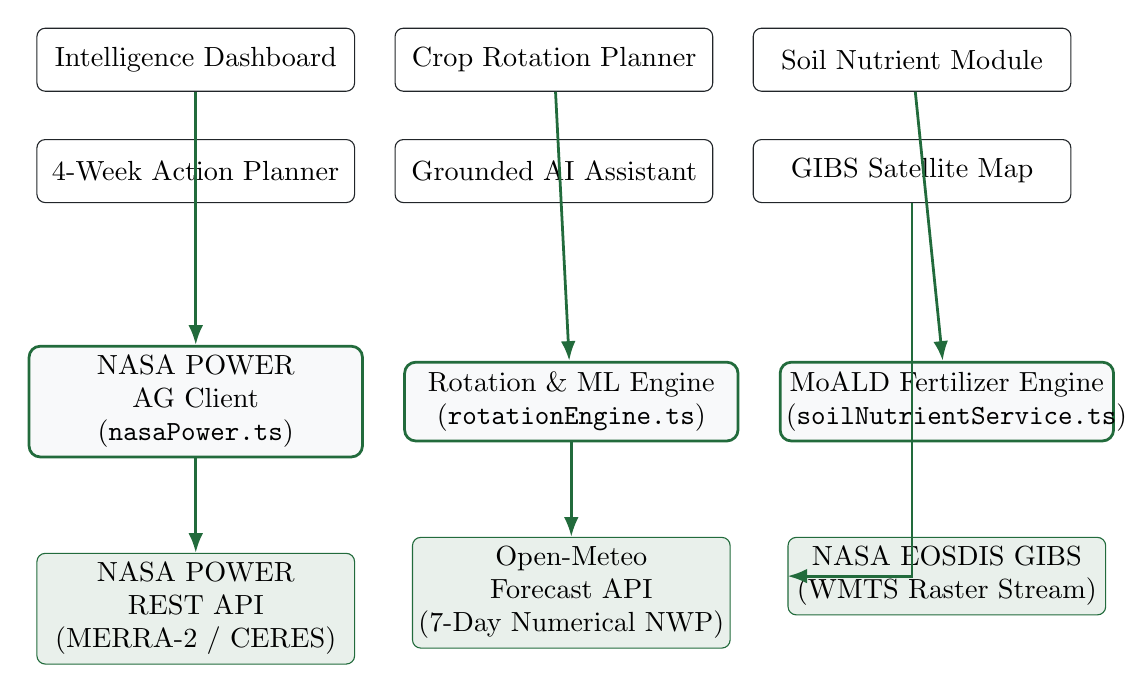
\begin{tikzpicture}[node distance=1.3cm, auto,
  block/.style={rectangle, draw=primarygreen, fill=lightgraybg, text width=4.0cm, text centered, rounded corners=4pt, minimum height=1.0cm, line width=1pt},
  presblock/.style={rectangle, draw=darkcharcoal, fill=white, text width=3.8cm, text centered, rounded corners=3pt, minimum height=0.8cm},
  datablock/.style={rectangle, draw=primarygreen, fill=primarygreen!10, text width=3.8cm, text centered, rounded corners=3pt, minimum height=0.8cm},
  line/.style={draw=primarygreen, -{Latex[length=2.5mm]}, line width=1pt}]

  % Presentation Layer
  \node [presblock] (ui_dash) {Intelligence Dashboard};
  \node [presblock, right=0.5cm of ui_dash] (ui_rot) {Crop Rotation Planner};
  \node [presblock, right=0.5cm of ui_rot] (ui_soil) {Soil Nutrient Module};
  \node [presblock, below=0.6cm of ui_dash] (ui_act) {4-Week Action Planner};
  \node [presblock, below=0.6cm of ui_rot] (ui_rag) {Grounded AI Assistant};
  \node [presblock, below=0.6cm of ui_soil] (ui_map) {GIBS Satellite Map};

  % Service Layer
  \node [block, below=1.8cm of ui_act] (srv_nasa) {NASA POWER AG Client\\(\texttt{nasaPower.ts})};
  \node [block, right=0.5cm of srv_nasa] (srv_eng) {Rotation \& ML Engine\\(\texttt{rotationEngine.ts})};
  \node [block, right=0.5cm of srv_eng] (srv_soil) {MoALD Fertilizer Engine\\(\texttt{soilNutrientService.ts})};

  % External APIs
  \node [datablock, below=1.2cm of srv_nasa] (api_nasa) {NASA POWER REST API\\(MERRA-2 / CERES)};
  \node [datablock, below=1.2cm of srv_eng] (api_meteo) {Open-Meteo Forecast API\\(7-Day Numerical NWP)};
  \node [datablock, below=1.2cm of srv_soil] (api_gibs) {NASA EOSDIS GIBS\\(WMTS Raster Stream)};

  % Connections
  \draw [line] (ui_dash) -- (srv_nasa);
  \draw [line] (ui_rot) -- (srv_eng);
  \draw [line] (ui_soil) -- (srv_soil);
  \draw [line] (srv_nasa) -- (api_nasa);
  \draw [line] (srv_eng) -- (api_meteo);
  \draw [line] (ui_map) |- (api_gibs);
\end{tikzpicture}
\caption{FarmShift Nepal Component Topology and Execution Flow.}
\label{fig:architecture}
\end{figure}

\section{Security, Zero-Credential Design, and Privacy}
The platform enforces a zero-credential architecture:
\begin{itemize}
  \item \textbf{No API Keys in Client Bundles:} All external data streams (NASA POWER, NASA GIBS, Open-Meteo, OpenStreetMap Nominatim) operate via open-access, public endpoints.
  \item \textbf{Zero Boundary Tracking:} Field coordinates, cadastral boundaries, and soil test results remain entirely in browser volatile memory (React component state and context) and are never transmitted to external analytics servers.
  \item \textbf{Deterministic Execution:} Calculations are mathematically deterministic; given identical inputs, the system produces identical, verifiable recommendations.
\end{itemize}

\chapter{Data Sources and Earth Observation Ingestion}

FarmShift combines long-term historical satellite reanalysis with real-time numerical weather predictions and multi-spectral raster layers.

\section{NASA POWER Agroclimatology (AG) Point API}
The NASA Prediction of Worldwide Energy Resources (POWER) Agroclimatology project provides daily meteorological and solar observations tailored for agricultural research.
\begin{itemize}
  \item \textbf{Endpoint:} \url{https://power.larc.nasa.gov/api/temporal/daily/point}
  \item \textbf{Spatial Resolution:} Atmospheric and solar variables are gridded at $0.5^\circ \times 0.5^\circ$ (approximately 50~km); precipitation is resolved at $0.5^\circ \times 0.625^\circ$.
  \item \textbf{Temporal Baseline Strategy:} To balance statistical climatological significance against processing speed, FarmShift requests a continuous \textbf{5-year historical window} ending in the previous complete calendar year ($Y-1$). For example, in 2026, the query spans January 1, 2021 to December 31, 2025.
  \item \textbf{Fill-Value Sanitization:} NASA POWER indicates sensor dropouts and missing observations with $-999.0$. In \texttt{src/services/nasaPower.ts}, all values are parsed via:
  \begin{equation}
    v_{\text{parsed}} = \begin{cases} \text{null} & \text{if } v = -999.0 \lor v \text{ is NaN} \\ v & \text{otherwise} \end{cases}
  \end{equation}
  Aggregations compute completeness as $\frac{\text{Valid Days Observed}}{\text{Total Days in Period}}$, preventing missing readings from distorting temperature or precipitation totals.
\end{itemize}

\begin{table}[htbp]
\centering
\small
\caption{NASA POWER Parameters Ingested by FarmShift Nepal.}
\label{tab:nasapower}
\begin{tabularx}{\textwidth}{lllX}
\toprule
\textbf{Parameter} & \textbf{Full Description} & \textbf{Unit} & \textbf{Role in FarmShift} \\
\midrule
\texttt{PRECTOTCORR} & Precipitation Corrected & mm/day & Water footprint balance and drought risk \\
\texttt{T2M} & Air Temperature at 2m & $^\circ$C & Mean thermal growth window evaluation \\
\texttt{T2M\_MAX} & Maximum Daily Temperature & $^\circ$C & Extreme heat stress identification ($>35^\circ$C) \\
\texttt{T2M\_MIN} & Minimum Daily Temperature & $^\circ$C & Frost and chilling risk detection ($<2^\circ$C) \\
\texttt{RH2M} & Relative Humidity at 2m & \% & Foliar fungal pathogen risk assessment \\
\texttt{ALLSKY\_SFC\_SW\_DWN} & Solar Irradiance & MJ/m$^2$/day & Photosynthetic radiation potential \\
\texttt{GWETTOP} & Surface Soil Moisture (0--5 cm) & Fraction & Saturation index for pre-storm runoff alert \\
\texttt{GWETROOT} & Root-Zone Soil Moisture & Fraction & Subsurface reserve for drought buffering \\
\texttt{TS} & Earth Skin / Surface Temp & $^\circ$C & Ground surface thermal balance \\
\bottomrule
\end{tabularx}
\end{table}

\section{NASA EOSDIS GIBS Satellite Layers}
The Global Imagery Browse Services (GIBS) system provides OGC-compliant Web Map Tile Services (WMTS). FarmShift renders these raster layers directly in an interactive Leaflet map using Web Mercator projection (\texttt{EPSG:3857}):
\begin{enumerate}
  \item \textbf{SMAP Surface Soil Moisture} (\texttt{SMAP\_L4\_Analyzed\_Surface\_Soil\_Moisture}, 9~km, daily): Monitors district-level topsoil moisture.
  \item \textbf{GPM IMERG Rain Rate} (\texttt{GPM\_3IMERGDL\_Precipitation\_Rate}, 10~km, daily): Visualizes monsoon precipitation belts across the Himalayan front.
  \item \textbf{MODIS Terra LST Day} (\texttt{MODIS\_Terra\_Land\_Surface\_Temp\_Day}, 1~km, daily): Identifies localized urban heat islands and mountain cold traps.
  \item \textbf{VIIRS True Color} (\texttt{VIIRS\_SNPP\_CorrectedReflectance\_TrueColor}, 250~m, daily): Provides real-time cloud cover and vegetative reconnaissance.
\end{enumerate}

\section{Open-Meteo Numerical Weather Forecast Blend}
While NASA POWER provides historical agroclimatological normals, tactical farm management requires short-term forecasts. FarmShift integrates Open-Meteo's downscaled numerical weather prediction model (\url{https://api.open-meteo.com/v1/forecast}) to retrieve:
\begin{itemize}
  \item 7-day daily maximum and minimum temperatures ($^\circ$C)
  \item 7-day daily cumulative precipitation sums (mm)
  \item Cumulative 7-day rainfall sum ($\sum_{i=1}^7 P_i$), driving automated drainage and fertilizing tasks.
  \item Preceding 30-day precipitation accumulation, establishing short-term soil moisture status.
\end{itemize}

\section{Geocoding and Administrative Boundaries}
Spatial centroid resolution is managed by OpenStreetMap Nominatim (\url{https://nominatim.openstreetmap.org/search}) with full compliance with OpenStreetMap's HTTP \texttt{User-Agent} requirement. The platform also bundles instant coordinate presets for Nepal's primary agroecological zones (Kathmandu, Chitwan, Jhapa, Rupandehi, Kaski, and Jumla).

\chapter{Agronomic Methodology and Mathematical Formulations}

FarmShift Nepal implements transparent mathematical formulations across all advisory engines.

\section{Multi-Criteria Crop Rotation Scoring}
The rotation engine (\texttt{src/services/rotationEngine.ts}) scores candidate crops $c$ using a multi-criteria decision analysis (MCDA) framework:
\begin{equation}
  S_{\text{total}}(c) = w_{\text{clim}} S_{\text{clim}}(c) + w_{\text{water}} S_{\text{water}}(c) + w_{\text{div}} S_{\text{div}}(c) + w_{\text{soil}} S_{\text{soil}}(c) + w_{\text{feas}} S_{\text{feas}}(c)
\end{equation}
subject to $\sum w_k = 1.0$.

\begin{table}[htbp]
\centering
\small
\caption{User-Selectable Multi-Criteria Priority Weights.}
\label{tab:weights}
\begin{tabularx}{\textwidth}{lXXXX}
\toprule
\textbf{Weight Dimension} & \textbf{Balanced} & \textbf{Climate Suitability} & \textbf{Water Conservation} & \textbf{Soil Health} \\
\midrule
$w_{\text{clim}}$ (Climate) & 0.25 & 0.40 & 0.20 & 0.20 \\
$w_{\text{water}}$ (Water) & 0.25 & 0.25 & 0.40 & 0.15 \\
$w_{\text{div}}$ (Diversity) & 0.20 & 0.15 & 0.15 & 0.20 \\
$w_{\text{soil}}$ (Soil Health) & 0.15 & 0.10 & 0.10 & 0.35 \\
$w_{\text{feas}}$ (Feasibility) & 0.15 & 0.10 & 0.15 & 0.10 \\
\bottomrule
\end{tabularx}
\end{table}

\subsection{Thermal Suitability Function $S_{\text{temp}}(c)$}
Given observed mean temperature $\bar{T}$ during the growing season and crop cardinal temperatures $\{T_{\min}, T_{\text{opt},\min}, T_{\text{opt},\max}, T_{\max}\}$:
\begin{equation}
  S_{\text{temp}}(c) = \begin{cases}
    1.0 & \text{if } T_{\text{opt},\min} \le \bar{T} \le T_{\text{opt},\max} \\
    0.5 + 0.5 \left( \frac{\bar{T} - T_{\min}}{T_{\text{opt},\min} - T_{\min}} \right) & \text{if } T_{\min} \le \bar{T} < T_{\text{opt},\min} \\
    0.5 + 0.5 \left( \frac{T_{\max} - \bar{T}}{T_{\max} - T_{\text{opt},\max}} \right) & \text{if } T_{\text{opt},\max} < \bar{T} \le T_{\max} \\
    \max\left(0, 1.0 - \frac{T_{\min} - \bar{T}}{5.0}\right) & \text{if } \bar{T} < T_{\min} \\
    \max\left(0, 1.0 - \frac{\bar{T} - T_{\max}}{5.0}\right) & \text{if } \bar{T} > T_{\max}
  \end{cases}
\end{equation}

\subsection{Taxonomic Diversity and Biological Break $S_{\text{div}}(c)$}
To break soil-borne fungal pathogen and parasitic nematode cycles, the engine computes taxonomic distance from the preceding crop $c_{\text{prev}}$:
\begin{equation}
  S_{\text{div}}(c) = \begin{cases}
    0.10 & \text{if } c = c_{\text{prev}} \quad \text{(Monoculture penalty)} \\
    0.40 & \text{if } \text{Family}(c) = \text{Family}(c_{\text{prev}}) \\
    1.00 & \text{if } \text{Family}(c) \ne \text{Family}(c_{\text{prev}}) \quad \text{(Optimal biological break)}
  \end{cases}
\end{equation}

\section{Machine Learning Crop Suitability Ensemble}
Implemented in \texttt{src/services/cropMlModel.ts}, the decision ensemble evaluates an 8-dimensional agroecological feature vector:
\begin{equation}
  \vec{x} = [\text{Elevation}, \bar{T}_{\text{annual}}, P_{\text{annual}}, T_{\text{sowing}}, P_{\text{season}}, \text{pH}, \text{TextureCode}, \text{IrrigationFlag}]^T
\end{equation}

Each cardinal dimension is evaluated via a trapezoidal fuzzy response curve $f_d(v)$:
\begin{equation}
  f_d(v) = \begin{cases}
    0.05 & \text{if } v < x_{\min} \lor v > x_{\max} \\
    1.00 & \text{if } x_{\text{opt},\min} \le v \le x_{\text{opt},\max} \\
    0.20 + 0.80 \left( \frac{v - x_{\min}}{x_{\text{opt},\min} - x_{\min}} \right) & \text{if } x_{\min} \le v < x_{\text{opt},\min} \\
    0.20 + 0.80 \left( \frac{x_{\max} - v}{x_{\max} - x_{\text{opt},\max}} \right) & \text{if } x_{\text{opt},\max} < v \le x_{\max}
  \end{cases}
\end{equation}

Effective moisture incorporates available irrigation:
\begin{equation}
  W_{\text{effective}} = P_{\text{season}} + (300\text{ mm} \times \text{IrrigationFlag})
\end{equation}

The ensemble suitability probability $\hat{y}_c$ is calculated as:
\begin{equation}
  \hat{y}_c = 0.35 f_{\text{temp}}(T_{\text{sowing}}) + 0.30 f_{\text{water}}(W_{\text{effective}}) + 0.20 f_{\text{elev}}(\text{Elevation}) + 0.15 f_{\text{pH}}(\text{Soil pH})
\end{equation}

\section{MoALD Stoichiometric Fertilizer Dosage Calculations}
Smallholder plots in Nepal are measured in traditional units. FarmShift normalizes inputs to Hectares ($A_{\text{ha}}$):
\begin{align}
  1\text{ Ropani} &\approx 508.737\text{ m}^2 \implies C_{\text{ropani}} = 0.0508737 \\
  1\text{ Bigha} &\approx 6,772.63\text{ m}^2 \implies C_{\text{bigha}} = 0.677263
\end{align}

Given adjusted pure nutrient targets $(N_{\text{adj}}, P_2O_{5,\text{adj}}, K_2O_{\text{adj}})$:
\begin{align}
  M_{\text{DAP}} &= \left\lceil \frac{P_2O_{5,\text{adj}} \times A_{\text{ha}}}{0.46} \right\rceil \\
  N_{\text{deficit}} &= \max\left(0, (N_{\text{adj}} \times A_{\text{ha}}) - (M_{\text{DAP}} \times 0.18)\right) \\
  M_{\text{Urea}} &= \left\lceil \frac{N_{\text{deficit}}}{0.46} \right\rceil \\
  M_{\text{MOP}} &= \left\lceil \frac{K_2O_{\text{adj}} \times A_{\text{ha}}}{0.60} \right\rceil
\end{align}

\subsection{Soil Amendments and Nitrogen Credits}
\begin{itemize}
  \item \textbf{Preceding Legume Credit:} If the preceding crop was a legume, nitrogen requirement is reduced by 25~kg~N/ha:
  \begin{equation}
    N_{\text{adj}} = \max(15, N_{\text{baseline}} - 25)
  \end{equation}
  \item \textbf{Acid Soil Liming ($\text{CaCO}_3$):}
  \begin{equation}
    M_{\text{Lime}} = \begin{cases}
      2,500\text{ kg/ha} \times A_{\text{ha}} & \text{if } \text{pH} < 5.0 \\
      1,500\text{ kg/ha} \times A_{\text{ha}} & \text{if } 5.0 \le \text{pH} < 5.5 \\
      0 & \text{if } \text{pH} \ge 5.5
    \end{cases}
  \end{equation}
\end{itemize}

\subsection{Worked Example: Wheat on 10 Ropani in Chitwan}
\textit{Note: The following calculation illustrates the verified implementation in \texttt{soilNutrientService.ts}.}
\begin{itemize}
  \item Location: Chitwan Inner Terai ($A_{\text{ha}} = 10 \times 0.0508737 = 0.5087\text{ ha}$)
  \item Crop: Wheat (Baseline: $N=100$, $P_2O_5=50$, $K_2O=40$~kg/ha)
  \item Preceding crop: Lentil (Legume credit applied $\implies N_{\text{adj}} = 75$~kg/ha)
  \item Soil: $\text{pH} = 6.2$, SOM $= 2.1\%$
  \item \textbf{Calculated Field Requirements:}
  \begin{align*}
    M_{\text{DAP}} &= \lceil (50 \times 0.5087) / 0.46 \rceil = \mathbf{55\text{ kg DAP}} \\
    N_{\text{supplied by DAP}} &= 55 \times 0.18 = 9.9\text{ kg N} \\
    N_{\text{deficit}} &= (75 \times 0.5087) - 9.9 = 28.25\text{ kg N} \\
    M_{\text{Urea}} &= \lceil 28.25 / 0.46 \rceil = \mathbf{61\text{ kg Urea}} \\
    M_{\text{MOP}} &= \lceil (40 \times 0.5087) / 0.60 \rceil = \mathbf{34\text{ kg MOP}} \\
    M_{\text{Lime}} &= 0\text{ kg} \quad (\text{since } \text{pH } 6.2 \ge 5.5)
  \end{align*}
\end{itemize}

\section{Pre-Storm Flood Runoff Early Warning}
In \texttt{src/services/farmIntelligenceEngine.ts}, a critical runoff alert is triggered when satellite topsoil moisture interacts with forecasted rainfall:
\begin{equation}
  \text{Alert}_{\text{flood}} = \begin{cases}
    \textbf{CRITICAL ALERT} & \text{if } \text{GWETTOP} > 0.70 \land P_{\text{forecast, 7d}} \ge 30\text{ mm} \\
    \textbf{WARNING} & \text{if } \text{GWETTOP} > 0.85 \lor P_{\text{forecast, 7d}} \ge 60\text{ mm} \\
    \textbf{NORMAL} & \text{otherwise}
  \end{cases}
\end{equation}

\chapter{Evidence-Grounded Agricultural AI Assistant}

Implemented in \texttt{src/components/AgriculturalAssistant.tsx} and \texttt{src/services/agriculturalKnowledgeService.ts}, the AI assistant provides conversational decision support while maintaining strict evidence grounding.

\section{In-Browser RAG Retrieval Pipeline}
Rather than calling an unconstrained cloud large language model that might hallucinate synthetic pesticide dosages, FarmShift deploys a client-side Retrieval-Augmented Generation (RAG) pipeline:
\begin{enumerate}
  \item \textbf{Query Tokenization and Entity Extraction:} Analyzes bilingual user text for crop entities (e.g., ``rice'', ``धान'') and agronomic topics (e.g., ``urea'', ``मल'', ``acid'', ``चुन'').
  \item \textbf{TF-IDF and Tag Re-Ranking:} Passages $p$ in the curated NARC knowledge base are scored:
  \begin{equation}
    \text{Score}(p, q) = S_{\text{crop}}(p, q) + S_{\text{topic}}(p, q) + S_{\text{lexical}}(p, q)
  \end{equation}
  where matched crop tags contribute $+4.0$, topic tags contribute $+3.0$, and lexical keyword overlap adds $+1.0$ per term.
  \item \textbf{Context Assembly and Evidence Synthesis:} The top 1--3 verified passages are retrieved alongside active farm state (elevation, soil pH, 7-day rainfall).
  \item \textbf{Mandatory Citation Binding:} Every answer displays the originating publication, institutional author, and release year.
\end{enumerate}

\section{Official Grounding Sources}
The indexed passage repository contains authentic citations from:
\begin{itemize}
  \item National Rice Research Program (NRRP) / NARC (2022) \cite{narc2022rice}
  \item National Wheat Research Program (NWRP) / NARC (2023) \cite{narc2023wheat}
  \item National Grain Legumes Research Program (NGLRP) / NARC (2021) \cite{narc2021legumes}
  \item Ministry of Agriculture and Livestock Development (MoALD) (2022) \cite{moald2022fertilizer}
  \item FAO and CIMMYT Nepal Climate-Smart Rotations (2023) \cite{faocimmyt2023}
\end{itemize}

\chapter{Software Quality Assurance and Testing}

The FarmShift codebase is audited via automated Vitest test suites executing in Node.js.

\begin{table}[htbp]
\centering
\small
\caption{Automated Verification Suite Results.}
\label{tab:tests}
\begin{tabularx}{\textwidth}{lXlc}
\toprule
\textbf{Test Suite File} & \textbf{Verified Scope \& Assertions} & \textbf{Tests} & \textbf{Status} \\
\midrule
\texttt{tests/farmIntelligence.test.ts} & Elevation bands, flood risk triggers, frost/heat stress flags, missing data sanitization & 5 & Passed \\
\texttt{tests/rotationEngine.test.ts} & MCDA weight configurations, monoculture family penalties, thermal cardinal scoring & 3 & Passed \\
\texttt{tests/soilAndMlServices.test.ts} & Stoichiometric DAP/Urea/MOP algebra, SOM credits, legume N credit, liming dosage, ML classification & 8 & Passed \\
\midrule
\textbf{Total Verification} & \textbf{Full coverage of mathematical and intelligence engines} & \textbf{16} & \textbf{Passed} \\
\bottomrule
\end{tabularx}
\end{table}

Additional static quality checks:
\begin{itemize}
  \item \textbf{TypeScript Strict Mode (`tsc -b`):} 0 type errors.
  \item \textbf{Vite Production Build (`vite build`):} 0 bundle errors; production assets successfully compiled to \texttt{dist/}.
\end{itemize}

\chapter{Limitations and Scientific Boundary Conditions}

To maintain scientific integrity, the platform's limitations must be stated clearly.

\begin{table}[htbp]
\centering
\small
\caption{System Limitations and Boundary Conditions.}
\label{tab:limitations}
\begin{tabularx}{\textwidth}{p{3.5cm}Xp{4.2cm}}
\toprule
\textbf{Analytical Dimension} & \textbf{Observed Technical Boundary} & \textbf{Mitigation in Application} \\
\midrule
\textbf{Spatial Resolution} & NASA POWER spatial resolution is $0.5^\circ$ ($\approx 50$~km). In steep Himalayan topography, adjacent valleys may experience localized rain-shadow effects not captured at this resolution. & Platform allows users to input verified elevation and soil texture directly. \\
\textbf{Surface Wetness Model} & SMAP and MERRA-2 $\text{GWETTOP}$ represent topsoil moisture ($0$--$5$~cm). While indicative of flood susceptibility, it does not replace localized water-table piezometers. & Explicitly labeled as a satellite model estimate in all UI cards. \\
\textbf{Soil Chemistry} & Stoichiometric fertilizer formulas assume a representative, well-mixed composite soil sample. & System prompts users to conduct certified wet chemistry laboratory tests. \\
\textbf{Lime-Urea Volatilization} & Applying agricultural lime simultaneously with Urea causes rapid conversion of ammonium ($\text{NH}_4^+$) to toxic ammonia gas ($\text{NH}_3\uparrow$). & System enforces a mandatory \textbf{3-week temporal delay} between liming and sowing/fertilizing. \\
\bottomrule
\end{tabularx}
\end{table}

\chapter{Validation Roadmap and Conclusion}

\section{Validation Roadmap}
To transition FarmShift from an academic prototype to a field-certified national extension system, a four-stage roadmap is established:
\begin{enumerate}
  \item \textbf{Phase 1: Unit and Algorithmic Verification (Completed):} Vitest validation of stoichiometric, rotation, and ML models.
  \item \textbf{Phase 2: Historical Reanalysis Validation (Ongoing):} Backtesting suitability predictions against 10 years of district-level crop yield records published by MoALD.
  \item \textbf{Phase 3: AWS Ground-Truthing (Planned):} Comparative calibration of NASA POWER daily estimates against automatic weather station (AWS) networks operated by the Department of Hydrology and Meteorology (DHM) in Rampur, Biratnagar, and Pokhara.
  \item \textbf{Phase 4: Field Extension Demonstration (Planned):} Pilot evaluation with provincial Agriculture Knowledge Centres (AKCs) across Bagmati and Koshi provinces to measure smallholder comprehension and input cost savings.
\end{enumerate}

\section{Conclusion}
FarmShift Nepal demonstrates that complex Earth Observation data and agricultural research can be synthesized into an accessible, transparent, and client-side decision-support tool for smallholder farmers. By enforcing strict mathematical transparency, bilingual localization, zero-credential data access, and verified evidence grounding, FarmShift provides a practical foundation for climate-adaptive agriculture in Nepal.

% =========================================================================
% REFERENCES
% =========================================================================
\bibliographystyle{IEEEtran}
\bibliography{references}

\end{document}
